\documentclass{article}
\usepackage{graphicx} % Required for inserting images

\title{Test 2}
\author{Tomáš Dudek}
\date{January 2025}

\begin{document}

\maketitle

\section{Introduction to Harmonic Oscillation}
It's a fundamental concept in physics and engineering. It describes an oscillatory motion with a force that reduces the amplitude over time.
The equation of motion for a damped harmonic oscillator is:
\[mx'' + cx' + kx = 0\]

where:
\begin{itemize}
    \item m is the mass
    \item c is the damping coefficient
    \item k is the spring constant
    \item x is displacement
    \item x' is velocity
    \item x'' is acceleration
\end{itemize}

The solution for the underdamped case (most common) is:
\[x(t) = Ae^{-{\gamma}t}cos(\omega't + \theta)\]
where:

\begin{itemize}
    \item A is the initial amplitude
    \item $\gamma = \frac{c}{2m}$ is the damping ratio
    \item $\omega' = \sqrt{\frac{k}{m} - {\gamma}^2}$ is the damped angular frequency
    \item $\theta$ is the phase angle
\end{itemize}

\section{Types of damping}
There are three main types of damping:

\begin{itemize}
    \item Underdamped: The system oscillates with decreasing amplitude over time. This occurs when $c^2 < 4mk$. This is the most common case in real systems, like a suspension bridge swaying after being disturbed.
    \item Critically damped: The system returns to equilibrium as quickly as possible without oscillating. This occurs when $c^2 = 4mk$. This is often desired in systems like door closers.
    \item Overdamped: The system returns to equilibrium without oscillating, but more slowly than the critically damped case. This occurs when $c^2 > 4mk$. Think of trying to move quickly through a thick fluid.
\end{itemize}

\section{Derivation of the formula}
Let's start with Newton's Second Law for a mass on a spring with damping:
\[F = ma\]
\[-kx - cx' = mx''\]  (negative signs because both forces oppose motion)
\[mx'' + cx' + kx = 0\]
To solve this second-order differential equation, we assume a solution of the form:
\[x(t) = e^{rt}\]
Substituting this into our differential equation:
\[mr^2e^{rt} + cre^{rt} + ke^{rt} = 0\]
\[e^{rt}(mr^2 + cr + k) = 0\]
Since $e^{rt} \neq 0$, we have the characteristic equation:
\[mr^2 + cr + k = 0\]
Using the quadratic formula:
\[r = \frac{-c \pm \sqrt{c^2 - 4mk}}{2m}\]

\section{Solving a problem}
Problem: A 0.5 kg mass is attached to a spring with spring constant k = 20 N/m. The system has a damping coefficient c = 1.0 Ns/m. If the mass is pulled 0.1 m from equilibrium and released from rest, find:
\begin{itemize}
    \item Whether the system is underdamped, critically damped, or overdamped
    \item The position as a function of time
    \item The time it takes for the amplitude to decrease to half its initial value
\end{itemize}
Let's solve this step by step:\\
1. First, let's determine the type of damping:
Calculate $c^2 - 4mk$
\[c^2 = 1.0^2 = 1.0 N^2s^2/m^2\]
\[4mk = 4(0.5 kg)(20 N/m) = 40 kgN/m\]
Since $1.0 < 40$, the system is underdamped.\\

\noindent 2. For the underdamped case:
\[\gamma = \frac{c}{2m} = \frac{1.0}{2(0.5)} = 1.0 s^{-1}\]
\[\omega_0 = \sqrt{\frac{k}{m}} = \sqrt{\frac{20}{0.5}} = 6.32 rad/s\]
\[\omega ' = \sqrt{\omega_0^2 - \gamma^2} = \sqrt{40 - 1} = 6.24 rad/s\]\\

\noindent 3. The position function is:
\[x(t) = 0.1e^{-t}\cos(6.24t)\]
using initial conditions: $x(0) = 0.1 m$, $x'(0) = 0$\\

\noindent 4. For half-amplitude:
\[0.1e^{-t_1} = 0.05\]
\[e^{-t_1} = 0.5\]
\[t_1 = ln(2) = 0.693 seconds\]

So after about 0.693 seconds, the amplitude will be half of its initial value.

\begin{figure}[h]
    \centering
    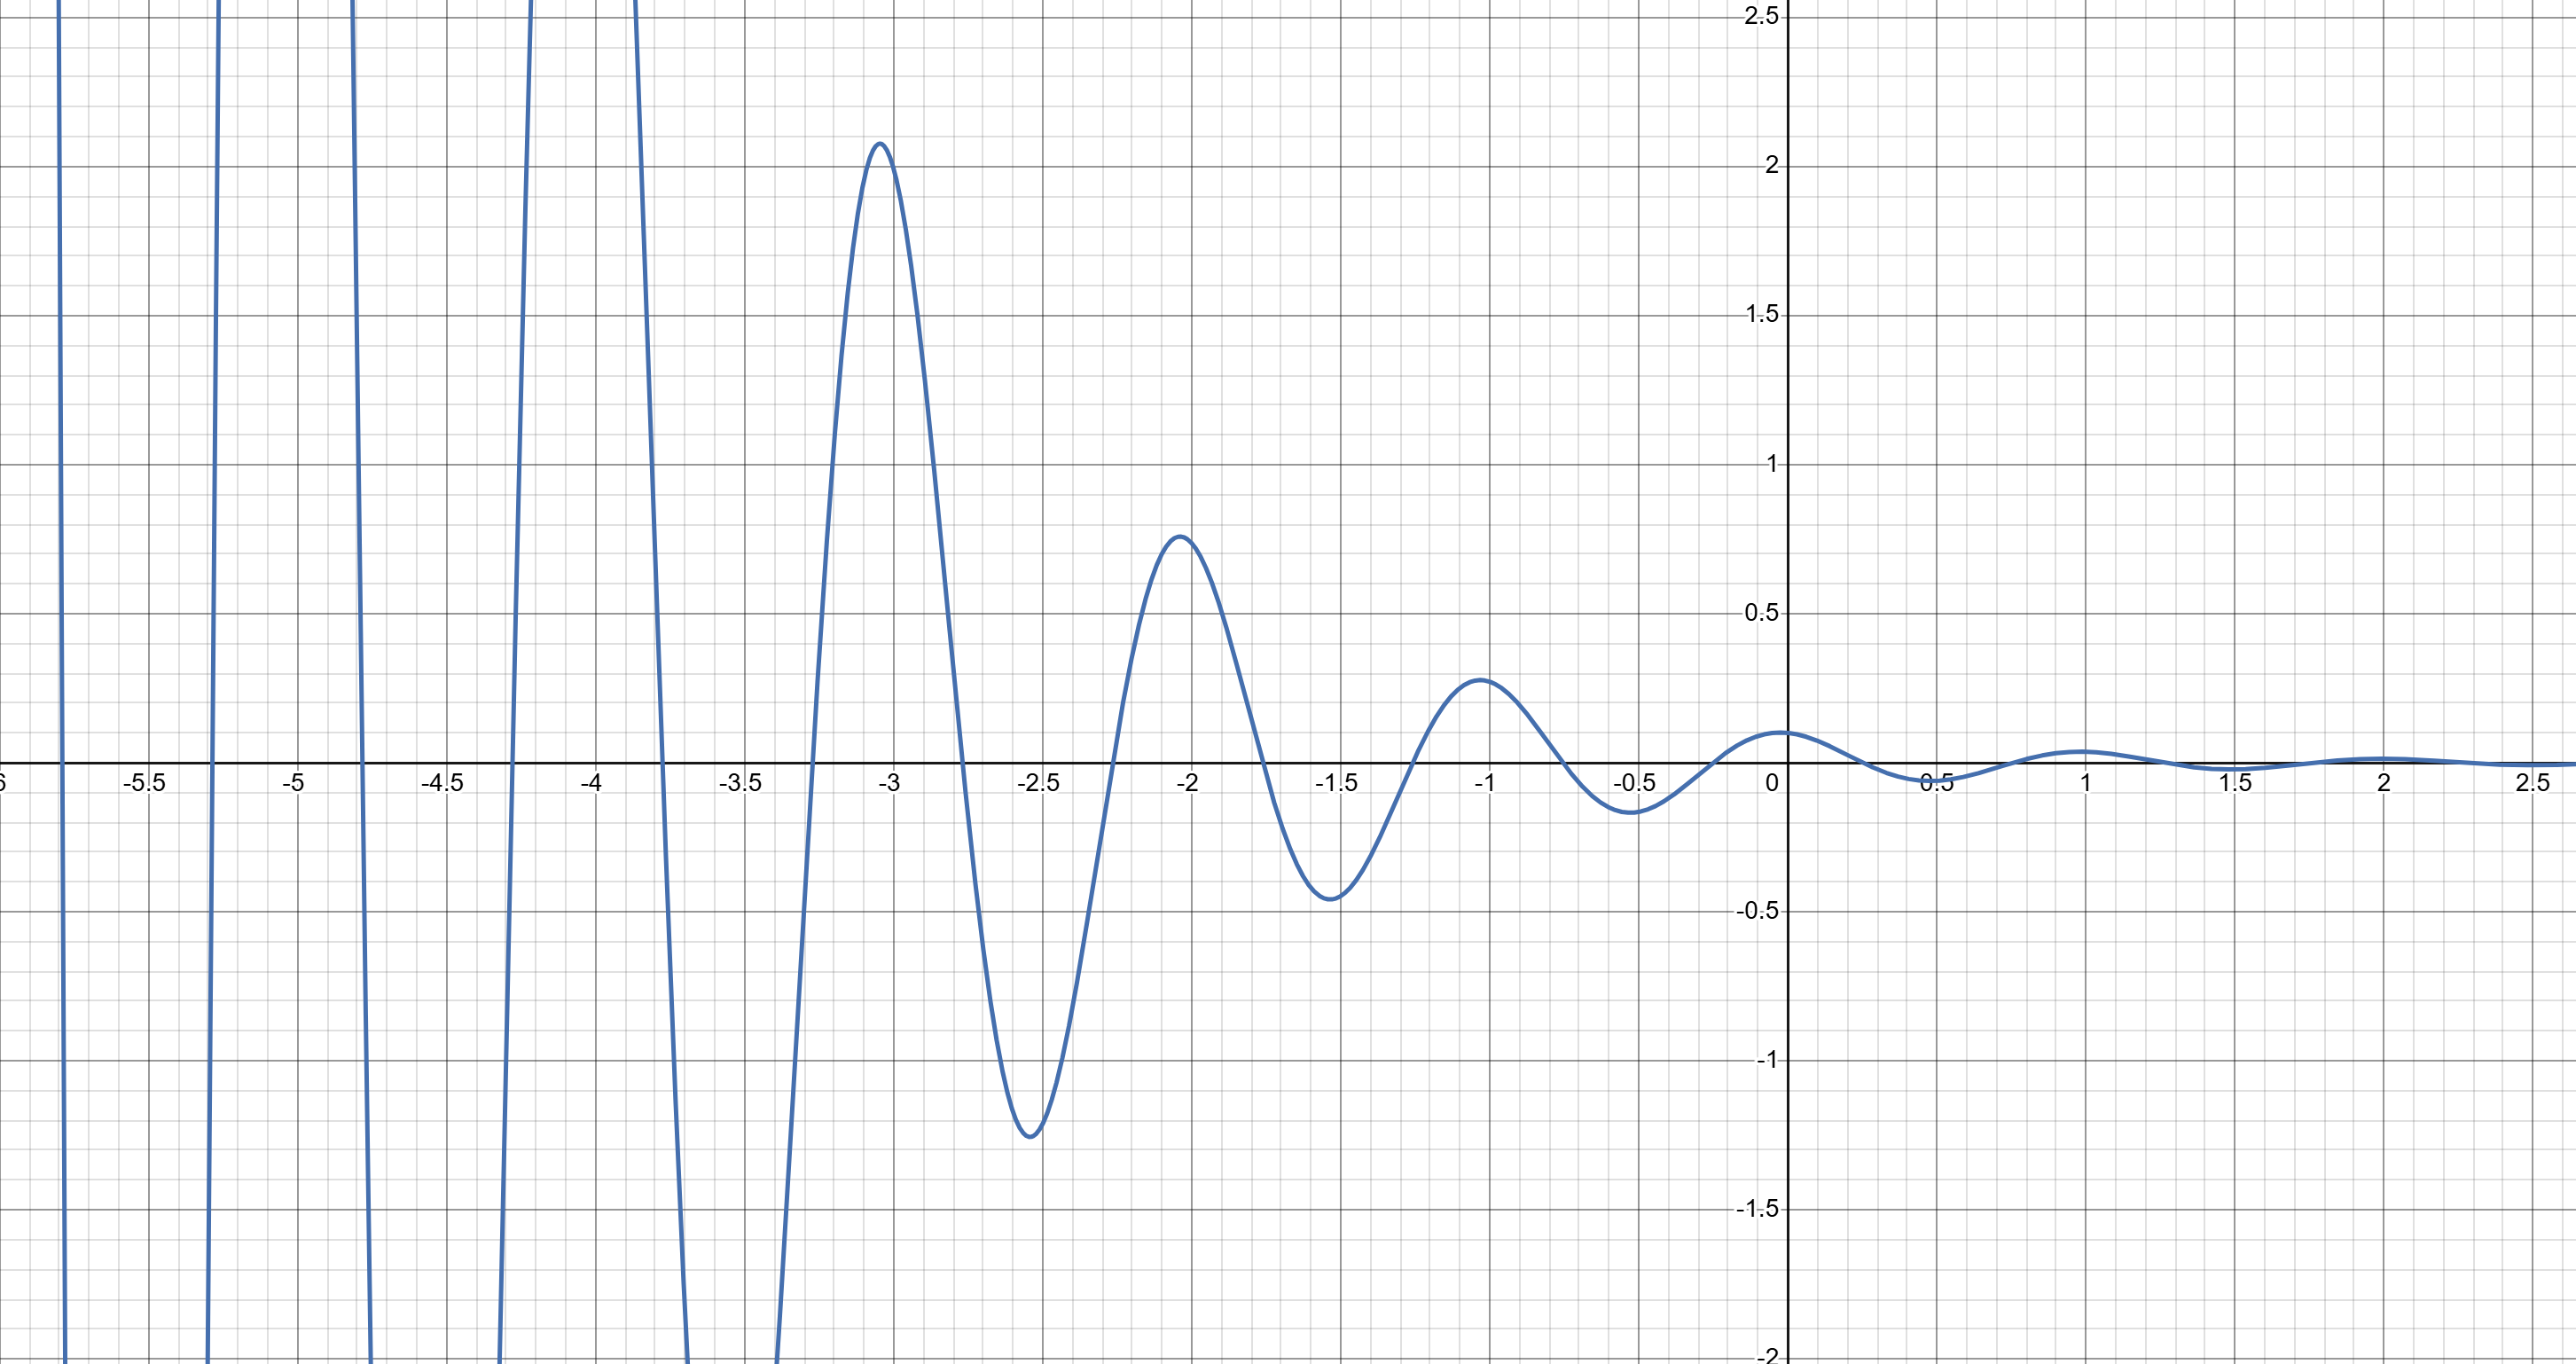
\includegraphics[width=1\linewidth]{Test2-Graph.png}
    \caption{Illustration of the problem in Desmos}
    \label{fig:enter-label}
\end{figure}
\end{document}
